\chapter{Supporting Information: Role of Nuclear Quantum Fluctuations on an electrochemical interface: the case of Pt(111) and water} \label{appendix5}

\section{Equilibration of the quantum kinetic energy for the clean and 0.5 ML H Pt(111)/water systems}

%\begin{figure}
%   \begin{center}
%    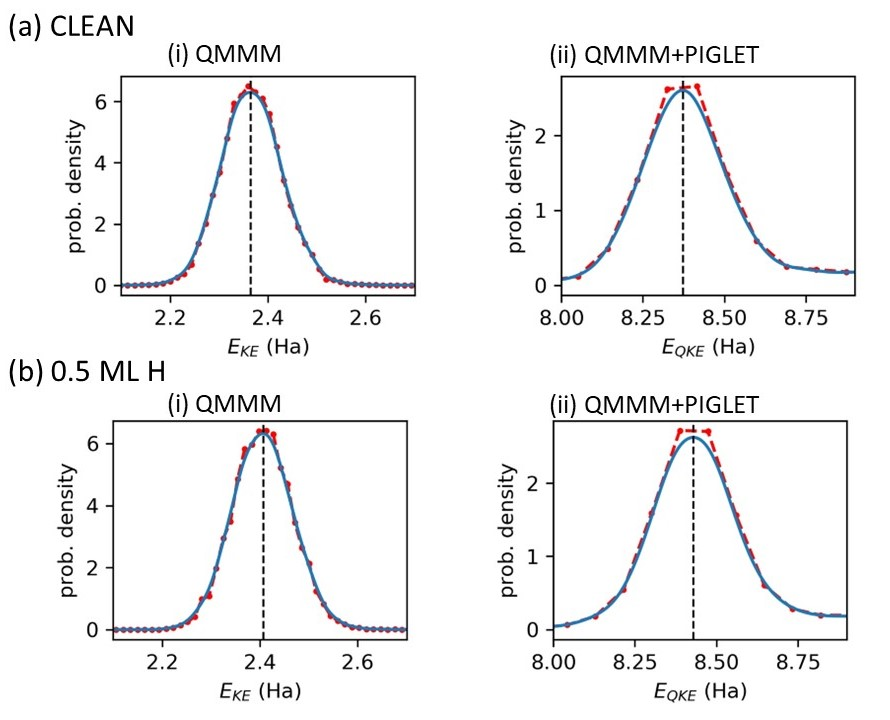
\includegraphics[width=14cm]{./Chapter3/figures/Slide13.JPG}       
%   \end{center}
%    \caption{The distribution of temperature for the (a) clean and (b) 0.5 ML system obtained from the equilibrated trajectories of (i) QMMM and (ii) QMMM $+$ PIGLET. The value of momenta in PIGLET simulations has no physical significance and therefore, the derived temperature which is just used as a sampling tool}
%  \label{fig:Slide13}
%\end{figure}

\begin{figure}
   \begin{center}
    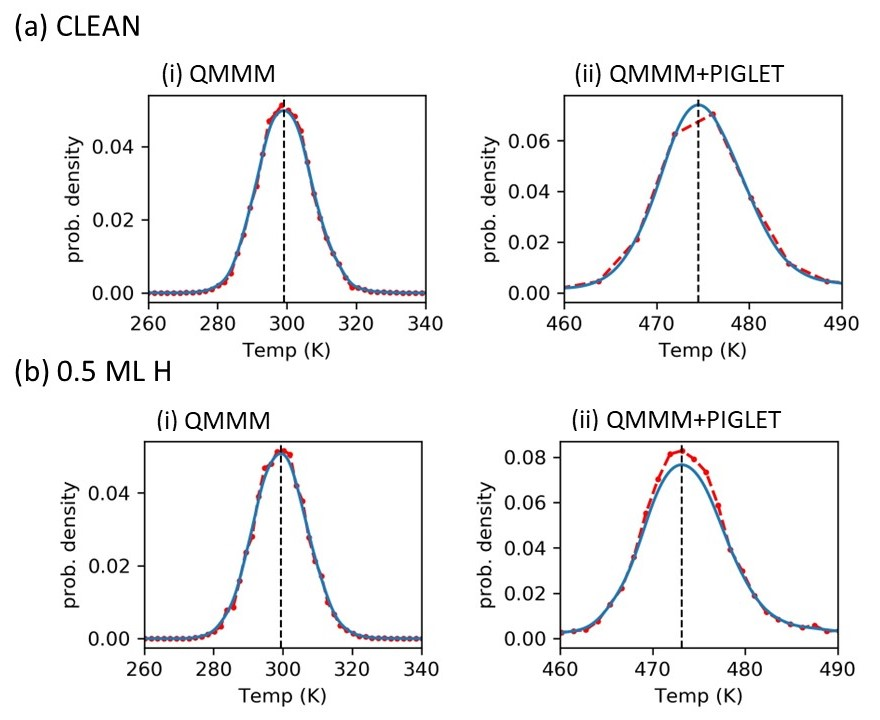
\includegraphics[width=14cm]{./Chapter3/figures/Slide14.JPG}       
   \end{center}
    \caption{The distribution of Kinetic energy for the (a) clean and (b) 0.5 ML system obtained from the equilibrated trajectories of (i) QMMM and (ii) QMMM $+$ PIGLET. It is to be noted that kinetic energy of the PIGLET simulation is the quantum kinetic energy which also includes the energy due to the inter bead harmonic interactions.}
  \label{fig:Slide14}
\end{figure}

Figure \ref{fig:Slide14} (a) and (b) are the distributions of quantum kinetic energy for the clean and 0.5 ML H systems respectively obtained from the (i) QMMM and (ii) QMMM $+$ PIGLET simulations. Each of the graphs has a Gaussian distribution in accordance with the sampling of the NVT ensemble. 

\section{Validation of QMMM + PIGLET}

In order to check the reliability of the results obtained from our novel implementation for QMMM $+$ PIGLET, we compare our results to the well established BOMD $+$ PIGLET simulation. Since the clean system has 1664 atoms, it is prohibitively expensive to do a full fledged BOMD $+$ PIGLET simulation. Therefore, we used a smaller model of the clean system having less number of atoms to compare the results of  QMMM $+$ PIGLET and BOMD $+$ PIGLET simulations. We call this system ``clean-small".

\subsection{System: clean-small}
The overall setup for the ``clean-small" system is the same as the larger system. The only difference is that a smaller supercell of (5x3) of the Pt surface is used. This results in 30 Pt atoms per layer and the total number of water molecules is reduced to 180. As a result, the width of the water film is decreased to 25 \AA{}. A representative snapshot for this smaller ``clean-small" system is shown in Figure \ref{fig:Slide15}(a).

\subsection{Comparison of results from (BOMD + PIGLET and QMMM + PIGLET)}

The validation of the QMMM $+$ PIGLET (w.r.t BOMD $+$ PIGLET) is done by comparing the important results which include the formation of interfacial bilayer and the dissociation of chemisorbed water. The formation and characteristics of the interfacial bilayer in the two simulations are depicted through the density profile in Figure \ref{fig:Slide15}(b). Similarly, the dissociation of chemisorbed water into adsorbed hydroxyl and solvated proton is portrayed through the joint distribution (Figure \ref{fig:Slide15}(c)) of the oxygen coordination number ($CN_O$) with respect to its normal distance from the Pt surface. The coordination number values of the oxygen atoms obtained from the BOMD $+$ PIGLET simulations agree with the QMMM $+$ PIGLET counterpart. Thus, our novel implementation of QMMM $+$ PIGLET passes the requisite validation. 

\begin{figure}
    \centering
    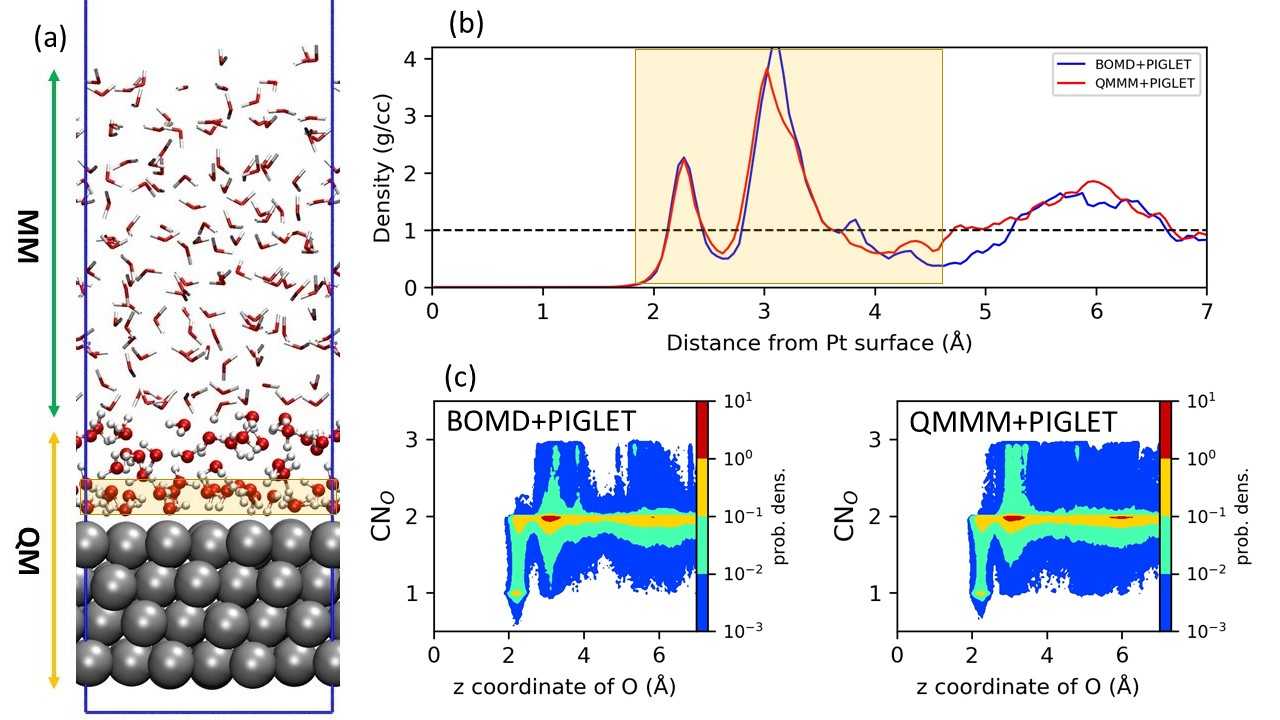
\includegraphics[width=14cm ]{./Chapter3/figures/Slide15.jpg}
    \caption{(a) A random snapshot of the smaller Pt(111)/water system (clean-small system) showing the QM and MM subsystems of the QMMM setup. (b) The planar energy of the water density (equation \ref{densitt}) as a function of its distance from the Pt surface along the surface normal obtained from BOMD $+$ PIGLET (blue) and QMMM $+$ PIGLET (red) simulations. (c) Joint distribution of the coordination number of oxygen ($CN_{O}$, described in Chapter 4) with its normal distance from the Pt surface obtained from the BOMD $+$ PIGLET (left) and QMMM $+$ PIGLET (right) simulations. }
    \label{fig:Slide15}
\end{figure}

